
\documentclass[
12pt, % Default font size, values between 10pt-12pt are allowed
%letterpaper, % Uncomment for US letter paper size
%spanish, % Uncomment for Spanish
UTF8
]{fphw}

% Template-specific packages
\usepackage{CTEX}
\usepackage[utf8]{inputenc} % Required for inputting international characters
\usepackage[T1]{fontenc} % Output font encoding for international characters
\usepackage{mathpazo} % Use the Palatino font

\usepackage{graphicx} % Required for including images

\usepackage{booktabs} % Required for better horizontal rules in tables

\usepackage{listings} % Required for insertion of code

\usepackage{enumerate} % To modify the enumerate environment

\usepackage[colorlinks,linkcolor=blue]{hyperref}

\usepackage{pythonhighlight}

%\usepackage {subcaption}

\usepackage{float}

\usepackage{subfigure}

\usepackage{caption}

%----------------------------------------------------------------------------------------
%	ASSIGNMENT INFORMATION
%----------------------------------------------------------------------------------------

\title{数据科学导论大作业} % Assignment title

\author{张晨阳 171180524} % Student name

\date{\today} % Due date

\institute{电子科学与工程学院} % Institute or school name

\class{数据科学导论} % Course or class name

%----------------------------------------------------------------------------------------

\begin{document}

\maketitle % Output the assignment title, created automatically using the information in the custom commands above

%----------------------------------------------------------------------------------------
%	ASSIGNMENT CONTENT
%----------------------------------------------------------------------------------------
\section{数据来源}
本报告所选取数据来源于Kaggle数据集,\footnote{https://www.kaggle.com/joelwilson/2012-2016-presidential-elections}该数据集包含美国各县的基本社会情况(种族结构,人口,经济等)及其在2012和2016年美国总统大选的投票数据。本次实践对美国各县的社会情况进行了一定的分析,并以此对总统大选结果进行分析与预测。\\
\textbf{作业压缩包中所含文件说明}
\begin{center}
	\begin{tabular}{|c|c|}
	\hline
	说明文档.pdf&本文件\\
	\hline
	.py文件 &源代码\\
	\hline
	.shx .shp .dbf文件&绘制地图所需的地理信息文件\\
	\hline
\end{tabular}
\end{center}

\section{预处理}
预处理代码位于文件pretreatment.py,定义了函数\emph{pretreatment()}进行预处理。具体步骤如下。
	\subsection{读取文件}
	采用pd.read\_csv()读取文件\\
	\begin{python}
		raw_data = pd.read_csv('../votes.csv')
	\end{python}
	\subsection{特征选择}
	原始数据的特征十分丰富,共有82列,每列特征具体含义可参见文件\emph{county\_facts\_dictionary.csv}。为了简化分析,选取了其中具有代表性一部分的数据,这一选取也是基于美国的社会文化情况做出的,例如因为种族和性别在美国社会中是很重要的议题,所以选取了大量种族结构和性别结构的特征。每列特征具体含义如下:
	\\
	\\
	\begin{tabular}{|c|c||c|c|}
		\hline
		state\_fips & 州编号 & votes\_dem\_2012 &奥巴马得票数 \\
		\hline
		state\_abbr & 州名缩写 & votes\_gop\_2012 & 罗姆尼得票数\\
		\hline
		county\_name & 县名 & age65plus & 年龄65岁以上人口比例 \\
		\hline
		population2014 & 2014年该县总人口 & SEX255214& 女性人口比例\\
		\hline
		votes\_dem\_2016 & 希拉里得票数&White&白人人口比例\\
		\hline
		votes\_gop\_2016 & 特朗普得票数&Black&黑人人口比例\\
		\hline
		Clinton & 希拉里得票率&Hispanic&西班牙裔人口比例\\
		\hline
		Trump & 特朗普得票率&RHI425214&亚裔人口比例\\
		\hline
		Edu\_batchelors&具有学士学位及以上人口比例&Income&人均收入(年)\\
		\hline
		Poverty & 贫困人口比例&&\\
		\hline
	\end{tabular}
\\
\\
	在这里可能存在着冗余的数据,比如得票数和得票率,但是因为后续的分析中有时需要用到得票数,有时需要用到得票率,且仅有两人的得票数算出的得票率与真实情况会存在一定偏差(由于还有其他政党及独立候选人的存在),所以两列数据都保留了。另外得票率在一定程度上也反映了该地区对这名候选人的支持率,下文统一用得票率进行称呼。
\\
\\
之后对一些列名进行了重命名使其意义更清晰,将百分数转为小数与其他数据统一格式,并以county\_name作为新的索引。
\begin{python}
	 columns=['state_fips','county_fips','state_abbr','county_name','population2014','votes_dem_2016', 'votes_gop_2016','Clinton', 'Trump',
	  'votes_dem_2012', 'votes_gop_2012','age65plus', 'SEX255214','White',
	  'Black','Hispanic', 'RHI425214','Edu_batchelors','Income','Poverty']
	data = raw_data[columns]
	data = data.rename(columns={'SEX255214':'Female'})
	data[['Female', 'Asian', 'age65plus','Edu_batchelors' ]] /= 100
	data = data.set_index('county_name')
\end{python}
	\subsection{检查数据缺失}
	因无数据缺失,故不用进行数据缺失处理\\
	\begin{python}
		print(data.isnull.sum())
		#data = data.dropna()
	\end{python}
	\subsection{建立新列}
	根据投票结果可以确定谁在该县赢得选举,新增两列\emph{result\_2016},\emph{result\_2012}表示选举结果,1代表民主党候选人获胜(希拉里,奥巴马),0代表共和党候选人获胜(特朗普,罗姆尼)
	\inputpython{pretreatment.py}{21}{24}
	\subsection{排序}
	同一个州内按照人口从多到少将县进行排序
	\inputpython{pretreatment.py}{25}{25}
	
	
\section{EDA 探索性数据分析}
	该部分代码位于文件eda.py
	\subsection{查看数据基本信息}:\\
	\inputpython{eda.py}{24}{26}
	\begin{figure}[H]
	\center{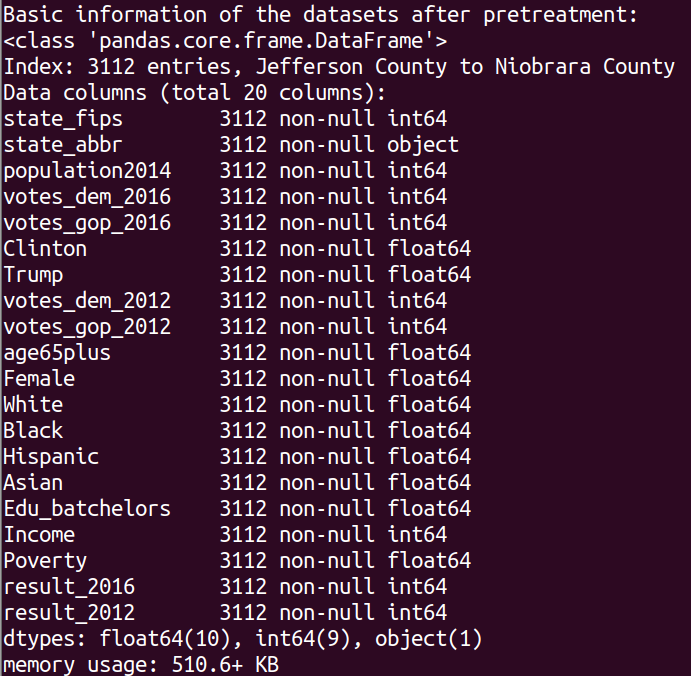
\includegraphics[scale = 0.4]{info.png}}
	\caption{数据集基本信息-1}
	\end{figure}
	\inputpython{eda.py}{31}{31}
	\begin{figure}[H]
	\center{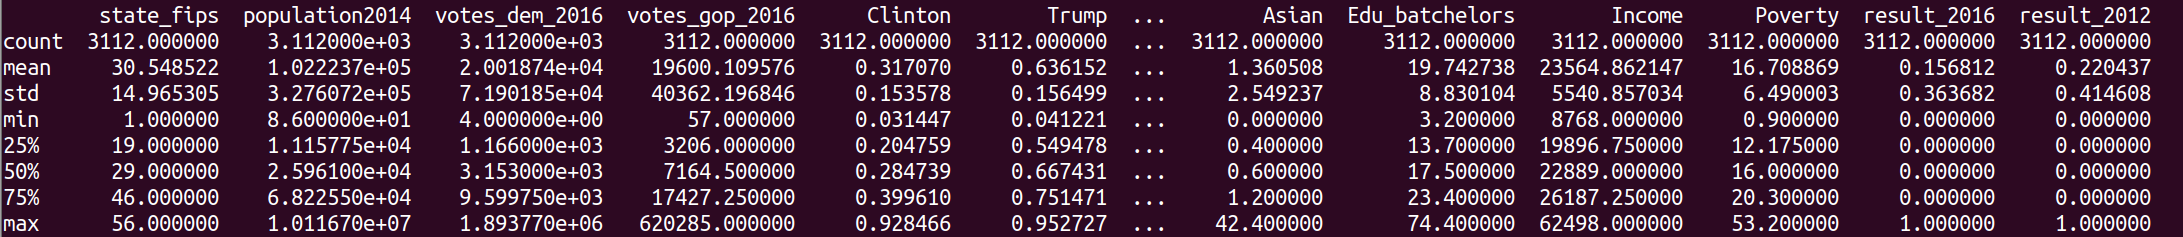
\includegraphics[scale = 0.45]{info2.png}}
	\caption{数据集基本信息-2}
	\end{figure}
	\subsection{查看数据相关性}
	通过seaborn库的热力图可以比较直观的表示数据间的相关关系\\
	\inputpython{eda.py}{28}{32}
	\begin{figure}[H]
	\center{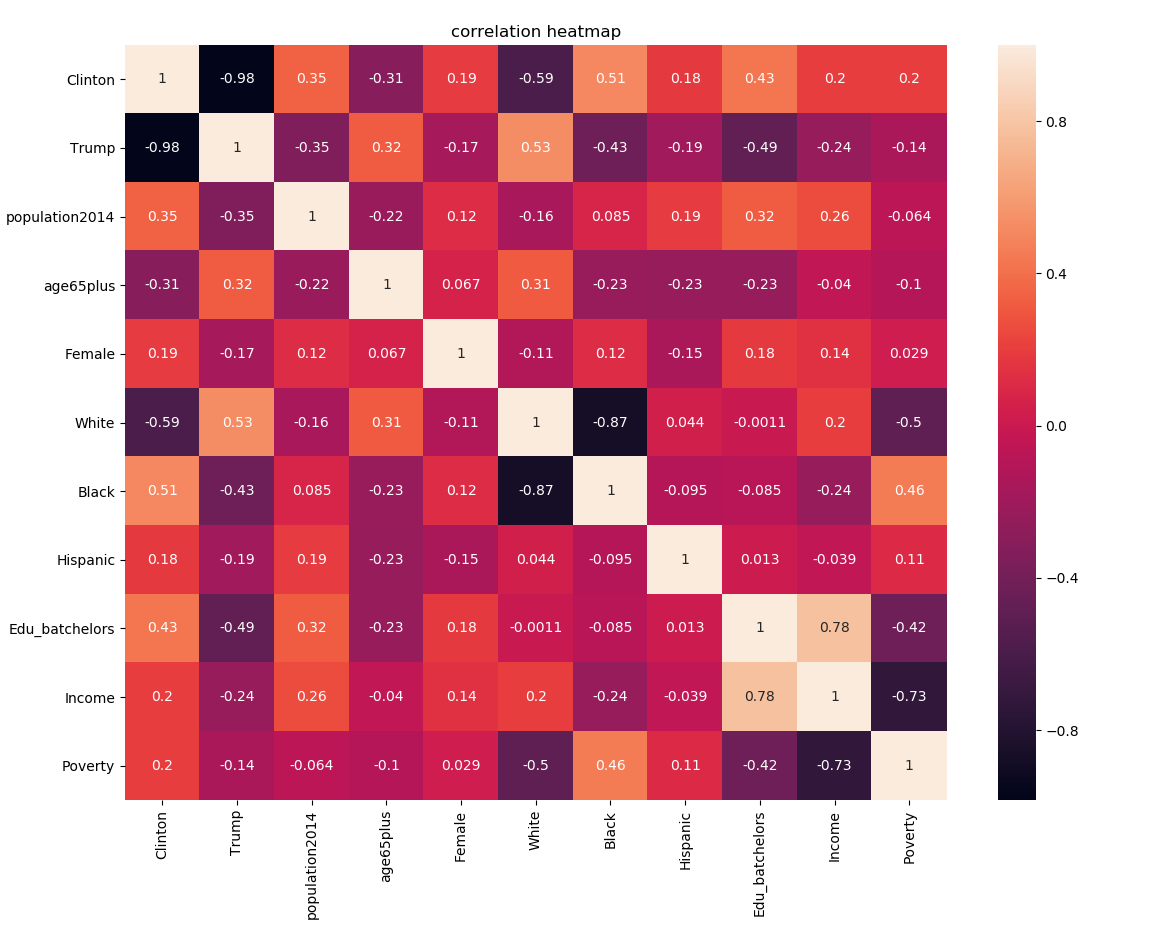
\includegraphics[scale = 0.6]{heatmap.png}}
	\caption{相关性热力图}
	\end{figure}
	\textbf{从图中可以看出:}
	\begin{enumerate}
		\item 部分属性之间存在着较强的相关关系,比如希拉里得票率和特朗普得票率之间负相关关系(这是必然的),还有人均收入与贫困率之间的负相关关系,这一情况也是符合常理的。
		\item 与种族有关的属性中,白人比例,黑人比例与得票率之间也有着比较强的相关关系,虽然0.5的相关系数在统计中不能说是很强,但考虑到选举受多种社会因素影响的,仅仅一个种族结构的特征有0.5的相关系数已经是比较显著了,这也印证了\emph{种族在美国政治中的重要性}。
		\item 女性与希拉里得票率之间的相关关系仅有0.19,比预期要低很多,一方面女性传统上倾向于支持民主党候选人,另一方面希拉里本身也是女性,理应更受女性欢迎,因此\emph{这一结果令人出乎意料。}
		\item 人口数量,受高等教育程度(学士学位拥有者)与希拉里得票率之间有着弱相关关系,这也是比较符合常理的。(大城市,高学历者倾向于支持民主党)
	\end{enumerate}

	从heatmap中找出相关系数较大的几个特征,通过pairplot作多变量图进一步观察数据间的关系:
	\inputpython{eda.py}{35}{38}
	\begin{figure}[H]
	\center{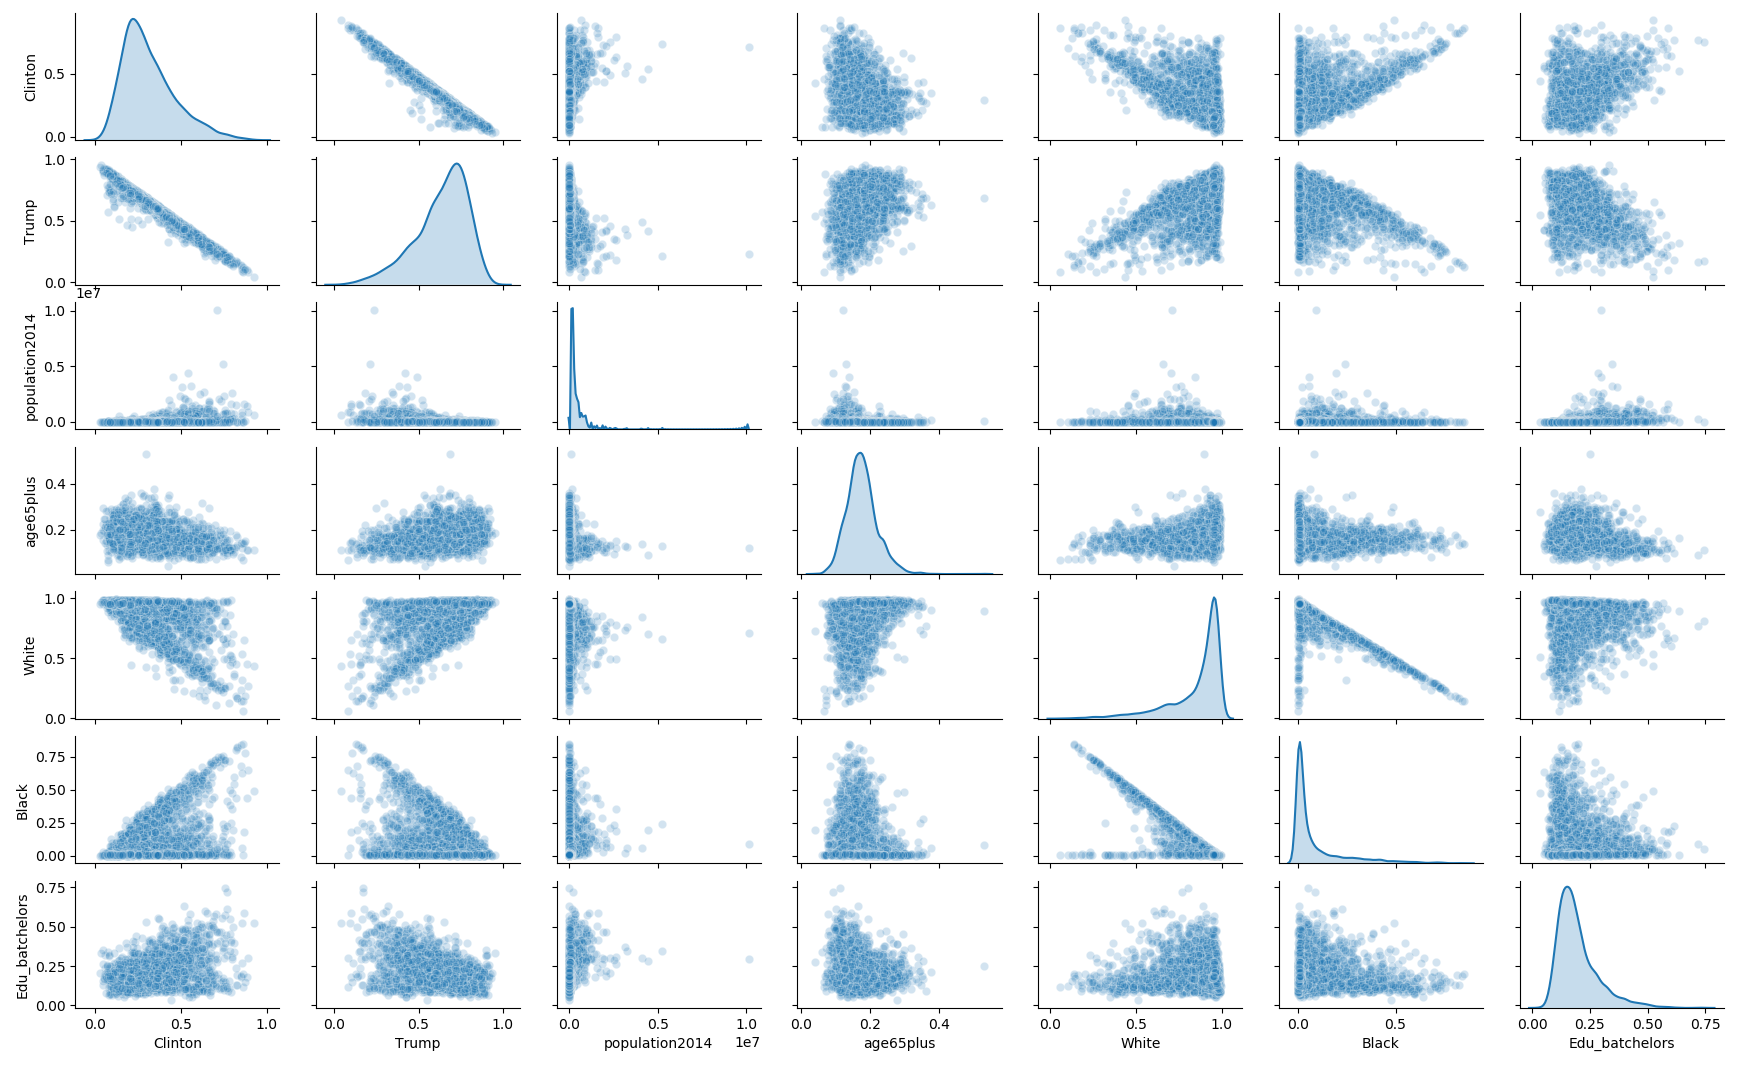
\includegraphics[scale = 0.38]{pairplot.png}}
	\caption{多变量图}
	\end{figure}
	从图中我们发现,或许是数据量太大的原因,许多特征间并没有很清晰的线性关系,在一些图中散点图是一团一团的,在一些图散点图呈现一种三角形状,即在x = 0和 y = 0附近聚集了大量离群值,除此之外呈现着线性关系。不过如果我们将数据细分到每个州,还是可以发现线性关系的,之后会进行展示。
	\subsection{观察特征分布情况}
	这里选用了箱型图观察美国各县的部分人群结构特征,选用箱型图的原因是因为可以比较直观的看出数据分散情况,分布是否不均衡。
	\inputpython{eda.py}{48}{63}
	\begin{figure}[H]
	\center{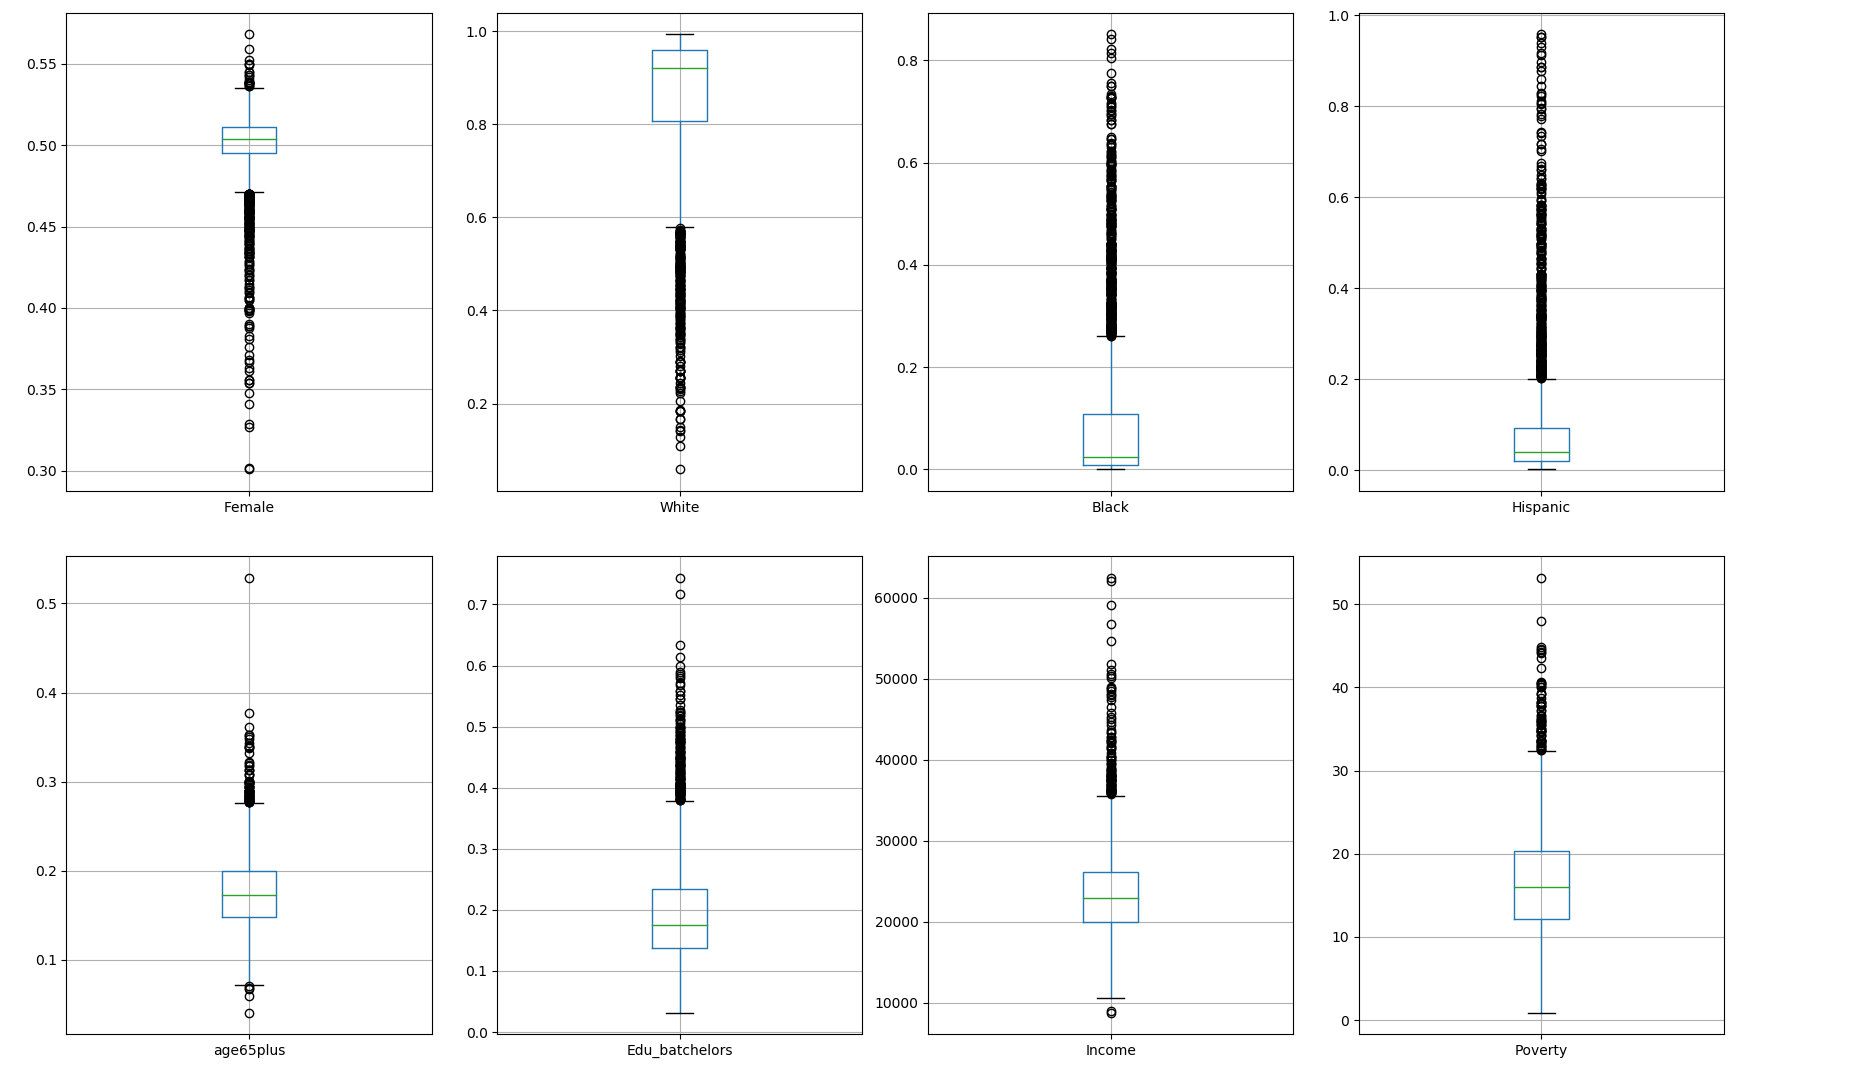
\includegraphics[scale = 0.51]{boxplot.png}}
	\caption{人群结构特征箱型图}
	\end{figure}
	从图中我们看出,以上特征均呈现分布不均衡的现象,有着大量离群值
	\begin{enumerate}
		\item 女性比例的箱型图还是比较正常的,大部分数据集中在0.5左右,两侧各有部分离群值。
		\item 白人属于多数族裔,在绝大部分县市都占大多数,黑人、西班牙裔在绝大多数县市占比较少,但在另一侧存在大量离群值,这也符合美国的种族结构。
		\item 从年龄分布可以看出美国存在一定的老龄化危机(国际上认为65岁以上人口占比超过7\%就存在老龄化问题)。
		\item 美国同样存在一定程度的贫富差距
	\end{enumerate}

	\subsection{封装打印统计特性的函数}
	这里定义了函数\emph{print\_result},可以打印出数据指定属性的各个统计特性,例如平均值,方差,中位数等
	\inputpython{eda.py}{7}{18}
	以人口为例,打印出人口数量的各项统计描述结果。
	\begin{python}
		 print_result(data, ['population2014'])
	\end{python}
	\begin{figure}[H]
		\centering
		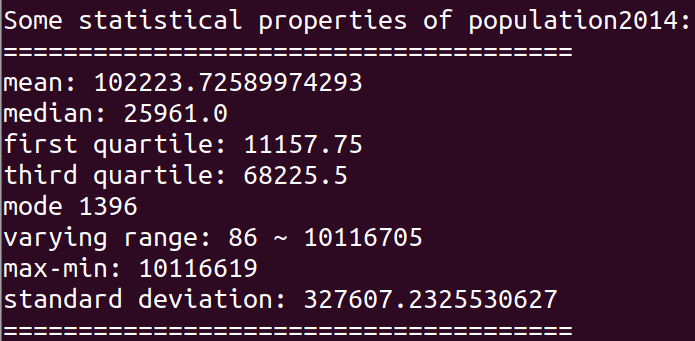
\includegraphics[scale = 0.7]{population.png}
		\caption{人口数量描述性统计结果}
	\end{figure}

	由此我们看出,美国人口的分布是非常的不均衡,第三四分位数接近7万人,而最大值却为1000万人,通过箱型图我们会有更加直观的感受。
	\begin{figure}[H]
		\centering
		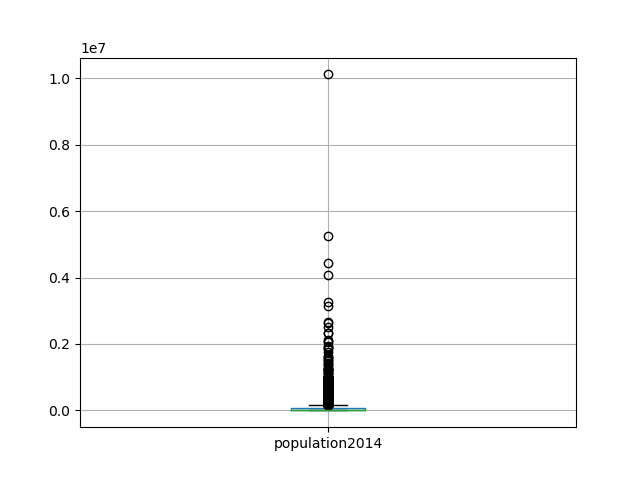
\includegraphics[scale =0.5]{p_box.png}
		\caption{人口数量箱型图}
	\end{figure}
	箱型图几乎都被压扁了,这说明在绝大多数县市,人口数量都是很稀少的,大部分人口集中在大城市,这一结论可以用来解释下一节发生的现象。
	\subsection{查看希拉里和特朗普获得总票数}
	对于选举来说,大家一定比较关心两位候选人最终得票数如何,以下结果会给出令人意想不到的事实。
	\begin{figure}[H]
	\center{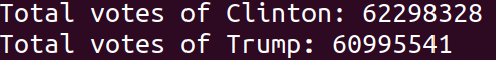
\includegraphics[scale = 0.8]{votes.png}}
	\caption{得票结果}
	\end{figure}
	\textbf{希拉里的总票数比特朗普多!}可以为什么现在的美国总统是特朗普呢,这是美国的选举制度导致的。美国的总统选举并不是直接普选,而是根据各州的人口和经济状况等分配给每个州一定票数,称为“选举人票”,赢得该州普选(即在该州得票最多)的候选人获得该州的全部选举人票,最后获得选举人票数最多的候选人即为新一任美国总统。赢了总票数却输了选举人票这一情况在美国发生过很多次,上一次发生在2000年(戈尔vs.小布什)。对于发生这一情况的原因,我做出的合理推测是,因为希拉里在一些州大幅度领先特朗普(称为深蓝州,例如加州,纽约州),但是无论她领先多少,她在该州获得的选举人票数是不变的,而在一些州特朗普以微弱优势赢了希拉里(称为摇摆州,例如:密歇根州,威斯康辛州),最终特朗普赢得了多数选举人票。
	\newpage
	\subsection{绘制选举结果地图}
	因为数据集中的信息是基于地理位置的,因此通过地图可以比较直观地看出选举结果与地理位置的关系。%下图中红色表示特朗普获胜,蓝色表示希拉里获胜。
	\begin{figure}[H]
		\centering
		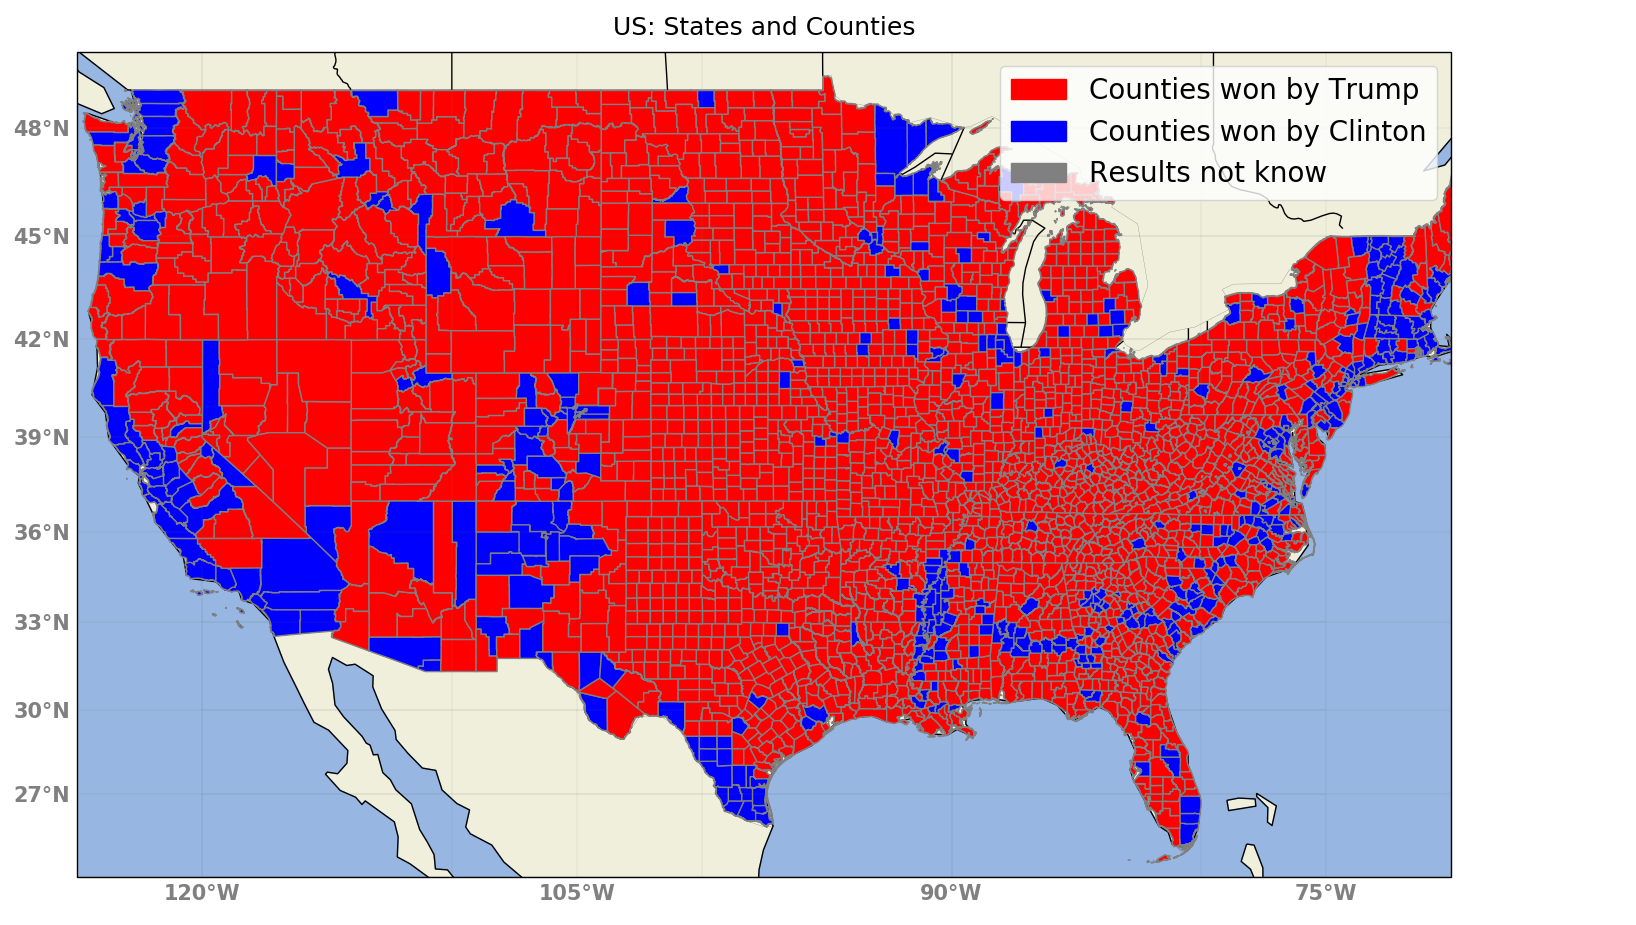
\includegraphics[scale = 0.7]{election_map.png}
		\caption{选举结果地图}
	\end{figure}
	从图中我们可以很明显地看出以下几个特征:(1)红色区域远远多于蓝色区域,也就是特朗普在绝大多数县都获得了多数票数。(2)蓝色区域主要集中在沿海等经济发达地区,尤其实西南部的加利福尼亚以及东北沿海(纽约州等)。\\
	  由此可以得出两个初步结论:
	\begin{enumerate}
		\item 美国人口分布很不均衡,有相当大部分人口集中在人口发达地区,而广大的内陆地区人口较少(与前几节中得到的结论相契合)
		\item 经济越发达的地区越倾向于支持希拉里,广大农业地区倾向于支持特朗普
	\end{enumerate}
	\subsection{绘制人口分布地图}
	图中颜色越深,表示人口越多。
	\begin{figure}[H]
		\centering
		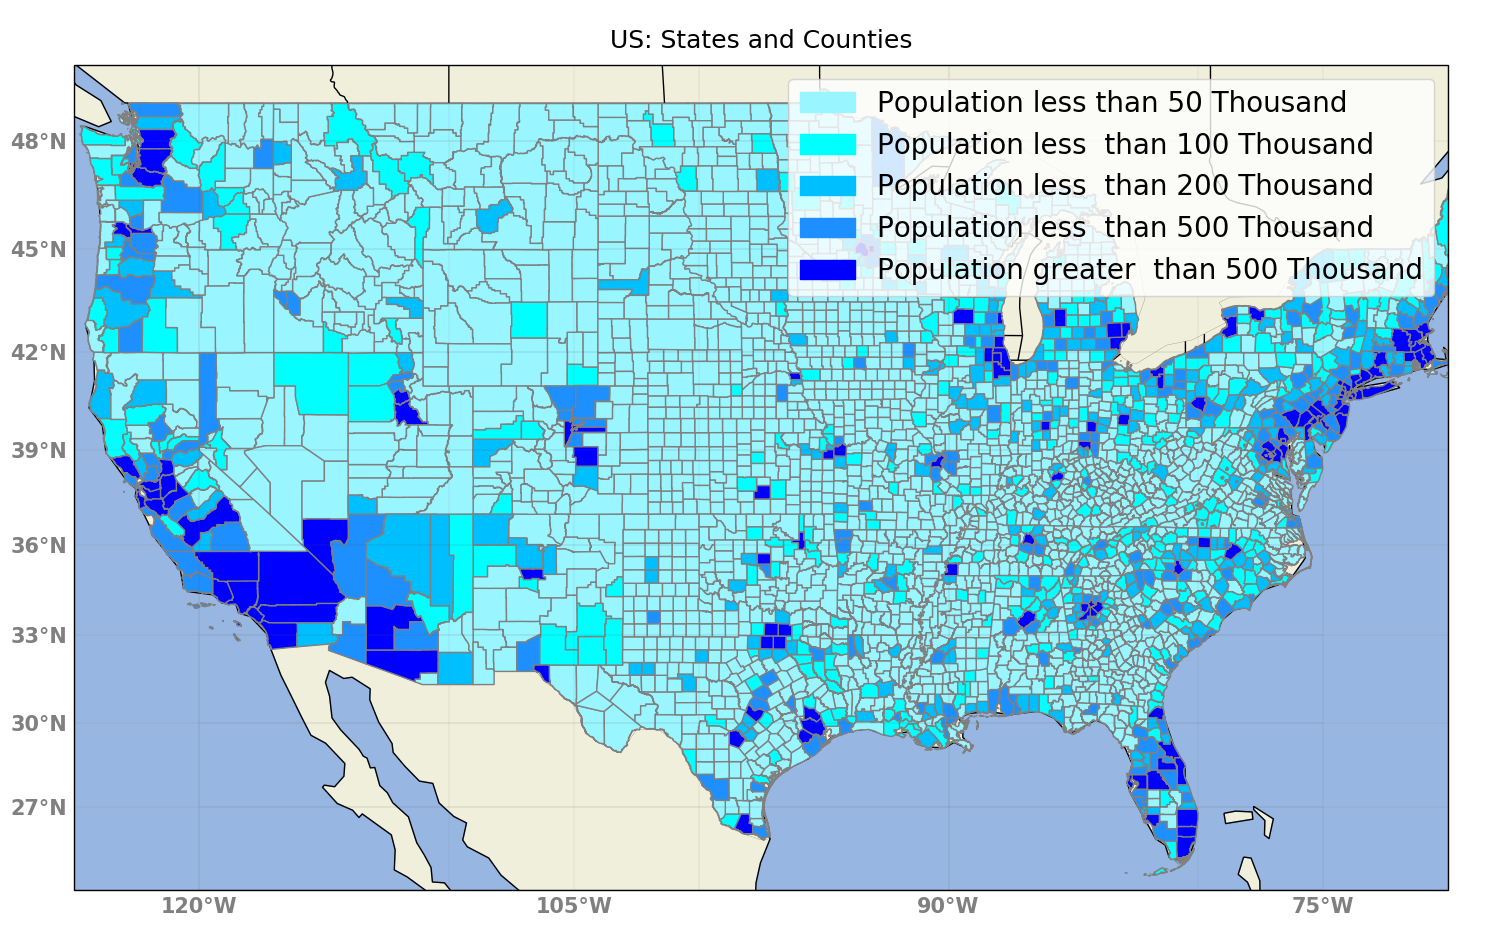
\includegraphics[scale = 0.7]{people_map.png}
		\caption{人口分布地图}
	\end{figure}
	将此图与选举地图相对比,我们发现两者具有较好的重叠性,即人口越多的地方相应着希拉里获胜的地方,这也进一步印证了我们的结论。同样我们也可以绘制其他特征的分布地图,由于篇幅限制,这里就不一一列出了。但是我们从图中仅能得出一些较为直观的感受,还需要通过具体数据进行进一步验证。	
	\subsection{}
	根据前述探索和已有经验,我们认为大城市(人口数量多),黑人,受过高等教育者更加支持希拉里,而白人比较不支持希拉里。\\
	通过探索各属性显著的前100个县中希拉里获胜的比例做出进一步结论\\
	\begin{python}
		print(data.sort_values(by = 'population2014', ascending = False).head(100).result_2016.sum()/100)
		print(data.sort_values(by = 'population2014', 
		ascending = False).head(100).population2014.sum()/data.population2014.sum())
		print(data.sort_values(by = 'population2014', ascending = False).tail(100).result_2016.sum()/100)
		print(data.sort_values(by = 'Female', ascending = False).head(100).result_2016.sum()/100)
		print(data.sort_values(by = 'Black', ascending = False).head(100).result_2016.sum()/100)
		print(data.sort_values(by = 'White', ascending = False).head(100).result_2016.sum()/100)
		print(data.sort_values(by = 'Edu_batchelors', ascending = False).head(100).result_2016.sum()/100)
	\end{python}
	\inputpython{eda.py}{89}{96}
	\begin{figure}[H]
		\subfigure[]{
		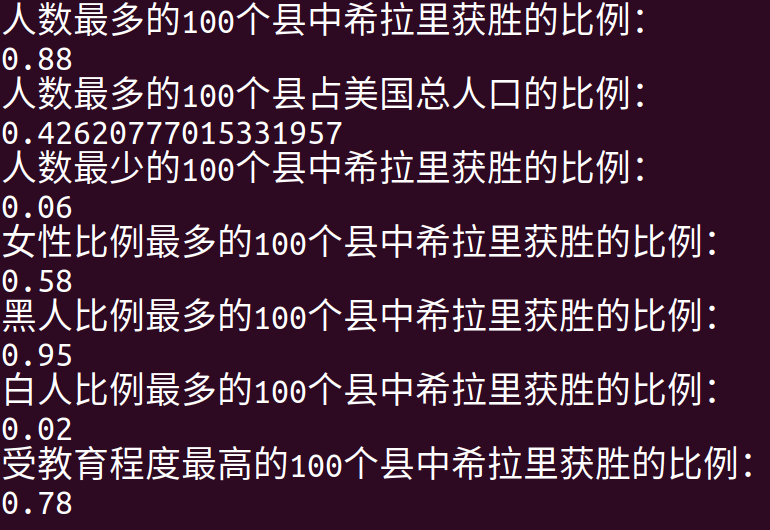
\includegraphics[scale = 0.65]{1.png}
	}
		\subfigure[]
		{
			\centering
			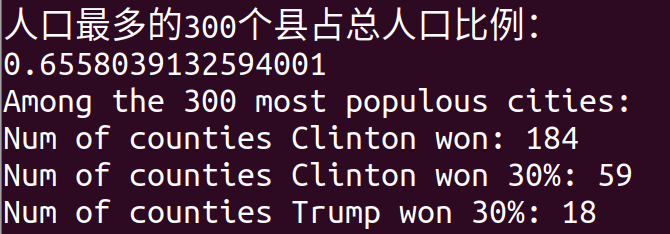
\includegraphics[scale = 0.4]{3.png}
		}
	\end{figure}
	希拉里在人口最多的100个县(占总人口43\%)中赢了88\%, 300个县(占总人口66\%)中赢了60\%多,其中有59个县大比例(30\%)领先特朗普,而特朗普仅有18个县大幅领先希拉里。这也印证了希拉里在大城市获得了压倒性支持并导致总票数高于特朗普。

	\subsection{细分数据}
	我们希望从州一级的数据中得到一些更清晰的结论。首先,州一级的数据应该更具有相关性,因为美国各州的经济、文化、政治等方面有着较大差异,若将全美国的数据放在一起由于多种因素的互相影响,我们不能得到比较清晰的结果,正如我们从pairplot图中观察到的。我们从总数据中选出三类数据,摇摆州数据,深红州数据,深蓝州数据。
	\inputpython{eda.py}{99}{104}
	\subsection{相关关系}
	通过探索发现,在深蓝州和摇摆州,受高等教育程度与希拉里得票率之间有着比较清晰的线性关系。这一发现可以在后续用来进行线性回归任务。
	\inputpython{eda.py}{106}{111}
	\begin{figure}[H]
		\centering
		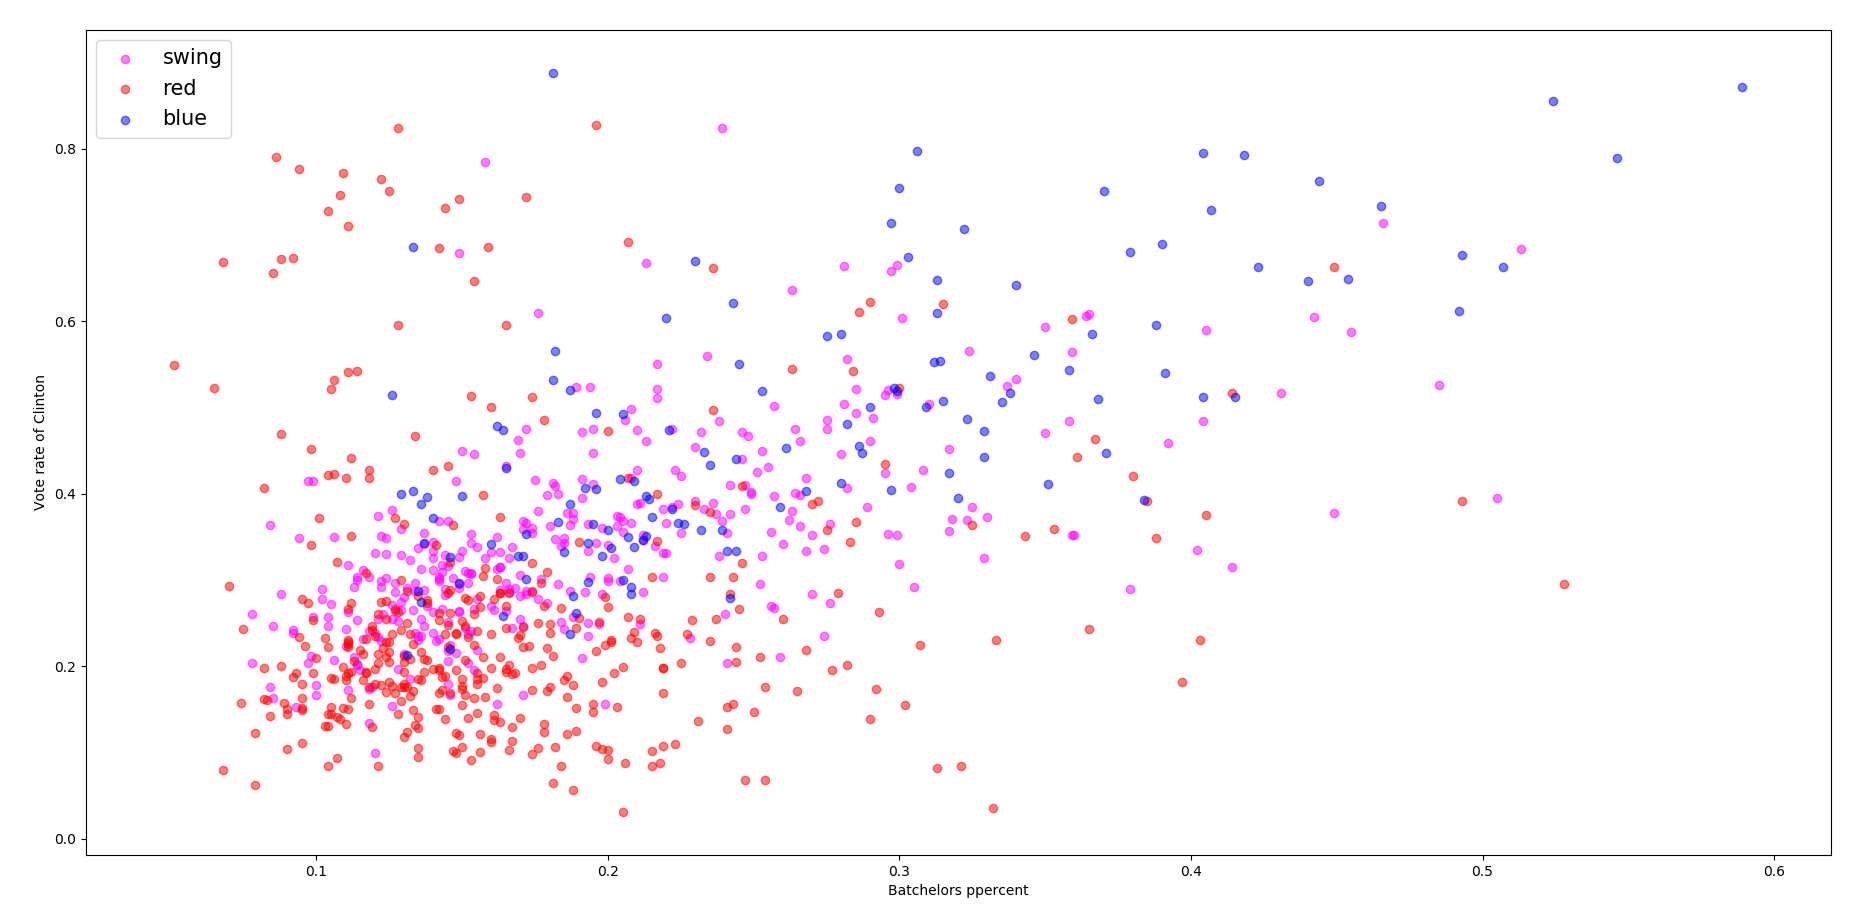
\includegraphics[scale=0.5]{bat_scatter.png}
		\caption{受高度教育程度与希拉里得票率散点图}
	\end{figure}
	深红州的数据呈现一团团的,有可能pairplot中的大量离群值是由于深红州数据造成的(猜测)。
	\subsection{得票率直方图}:\\
	\inputpython{eda.py}{115}{128}
	\begin{figure}[H]
		\centering
		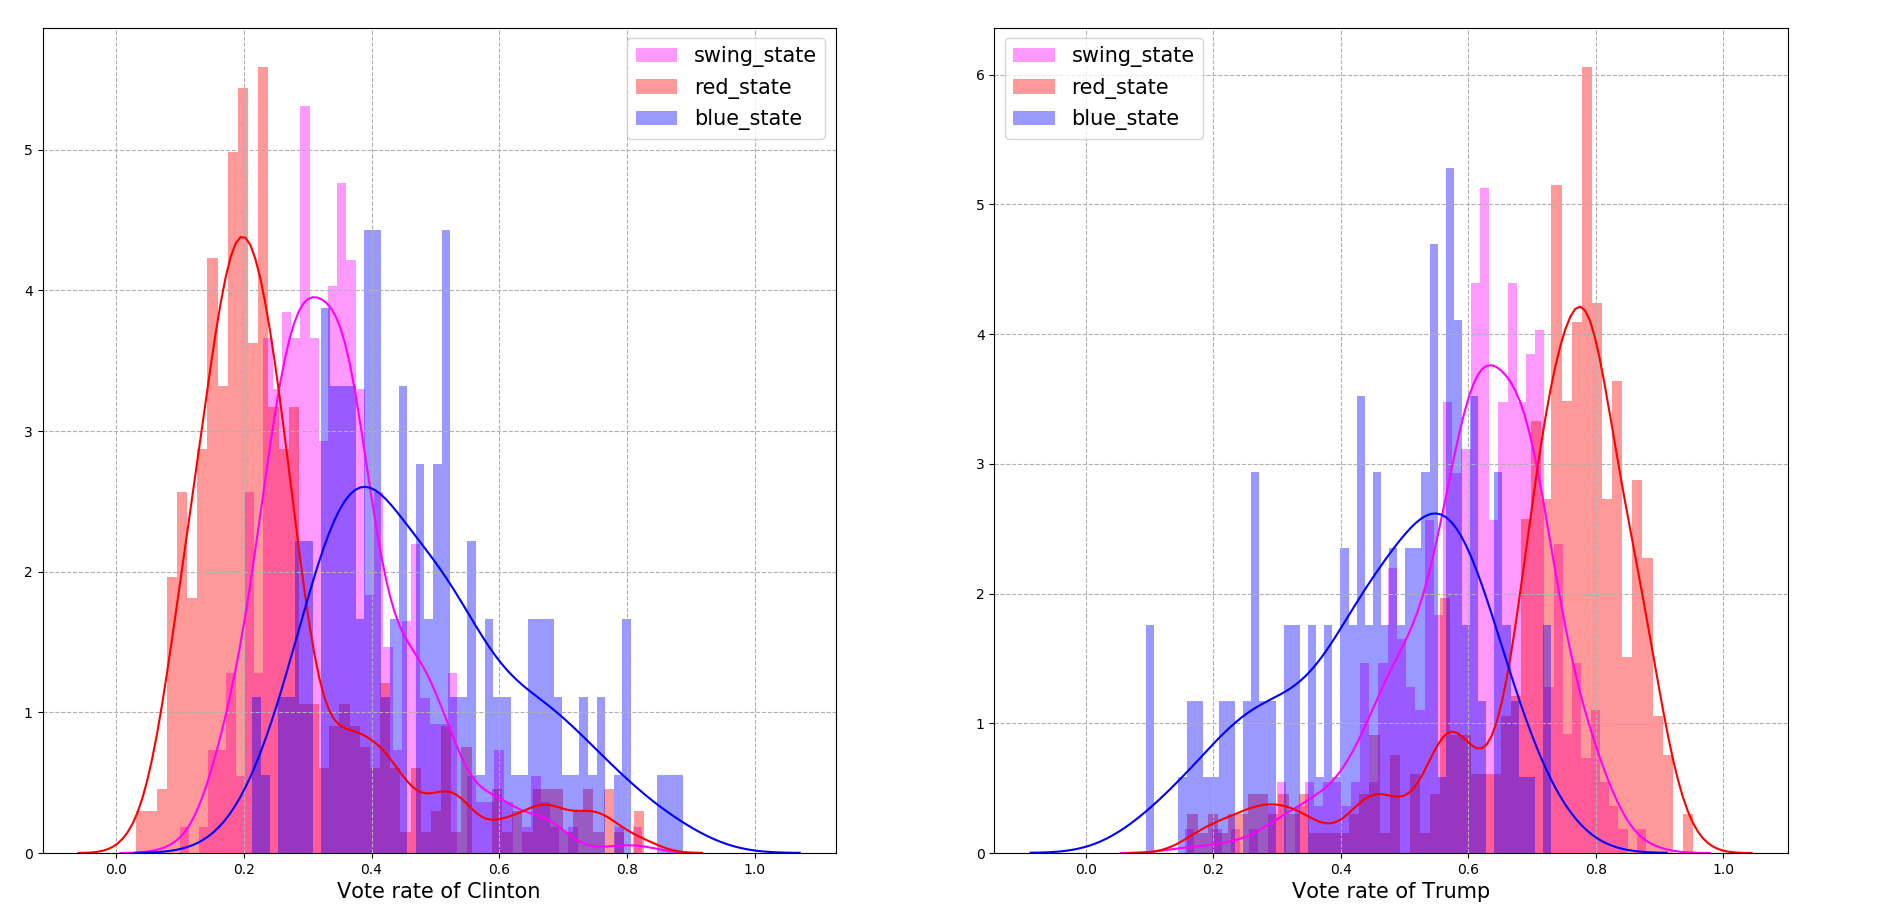
\includegraphics[scale=0.55]{vote_rate.png}
	\end{figure}
	从图中看出:
	\begin{enumerate}
		\item 深蓝州更加支持希拉里,深红州更加支持特朗普,摇摆州位于中间位置(符合先验知识)
		\item 深红州均值较大,方差较小,深红州人民团结一致支持特朗普?而深蓝州均值较小,方差较大,蓝州人民支持希拉里的程度似乎没有红州人民支持特朗普一样。(这也反映了希拉里败选的另一个原因,因为很多民主党选民讨厌希拉里,所以他们宁愿不投票)
		\item 特朗普在摇摆州更受支持,极大的可能正是因为摇摆州人民的支持使得特朗普当选
	\end{enumerate}


\section{统计推断}
在进行了EDA之后,选取其中一些数据进行统计推断。统计推断主要包括参数估计与假设检验,两者都是根据样本信息对总体的数量特征进行推断,但是角度不同。参数估计是以样本估计总体参数的真值,假设检验是以样本检验对总体参数的先验假设是否成立。
	\subsection{参数估计}
	该部分代码位于文件par\_estimate.py中。
		\subsubsection{点估计}
		选取深红州,深蓝州和摇摆州希拉里得票率数据做均值的点估计。
		\inputpython{par_estimate.py}{12}{29}
		\begin{figure}[H]
			\centering
			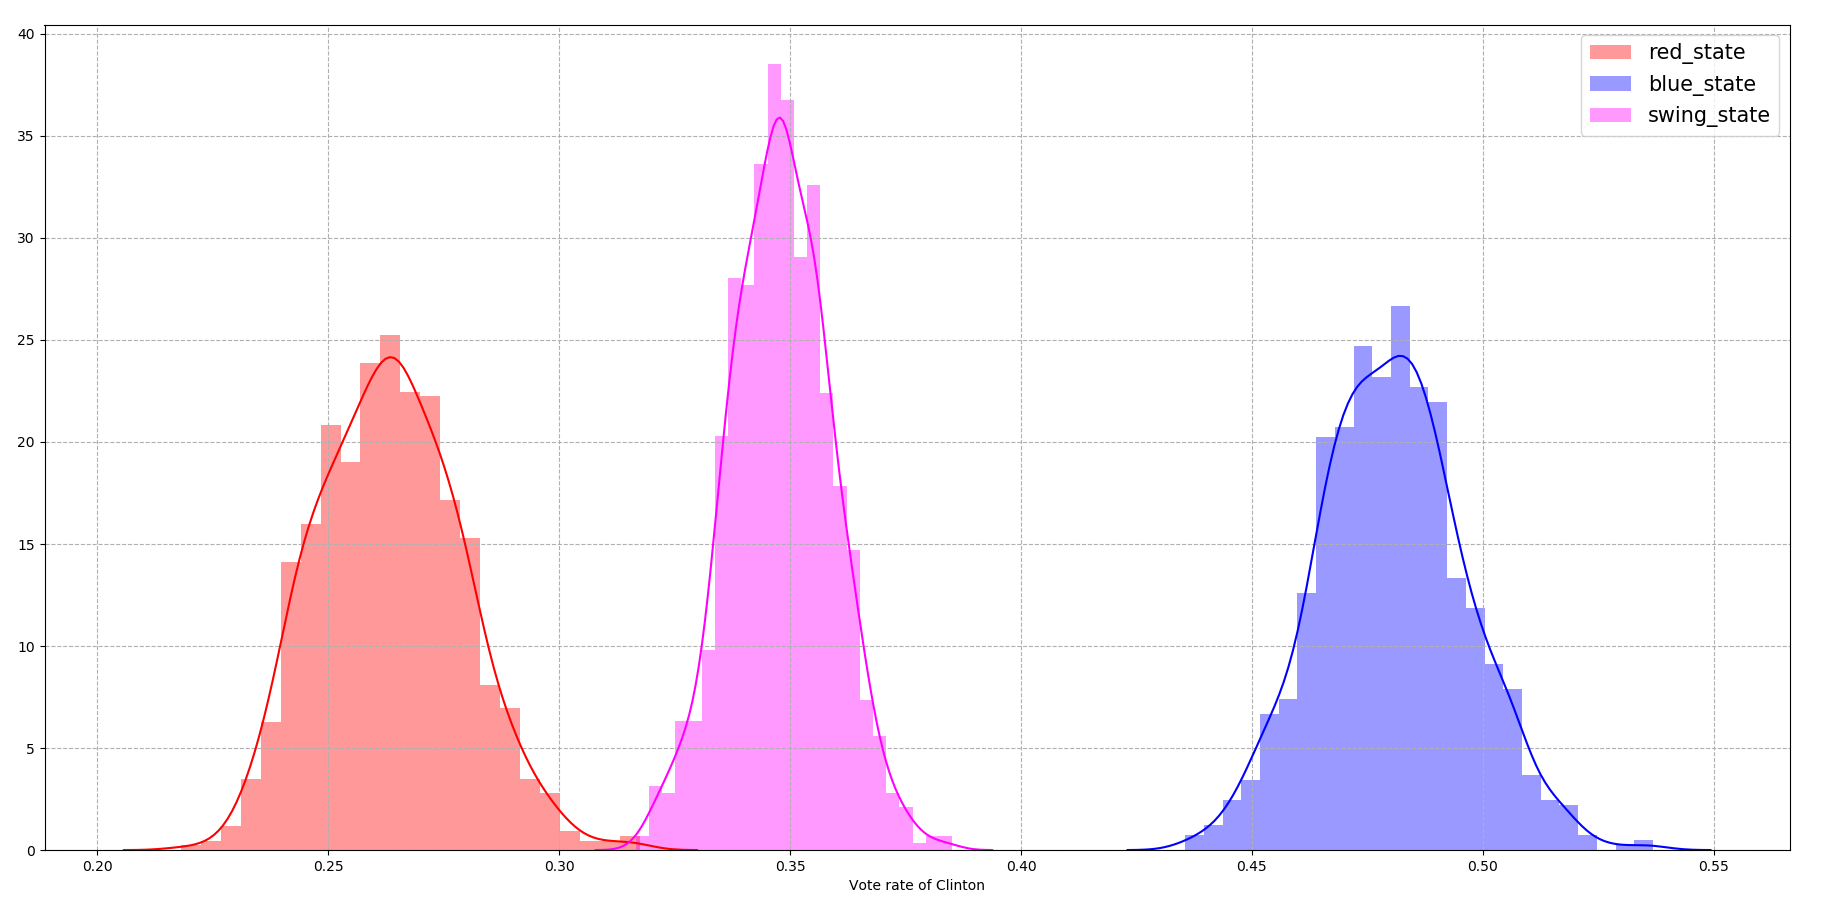
\includegraphics[scale=0.45]{pnt.png}
			\caption{样本均值的分布(希拉里)}
			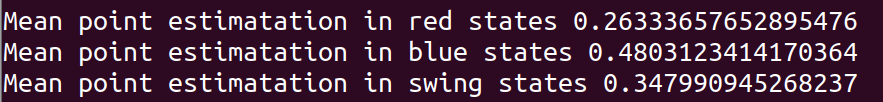
\includegraphics[scale=0.45]{pnt_1.png}
			\caption{点估计结果(希拉里)}
		\end{figure}
	即使在深蓝州希拉里得票率的均值的点估计值也未能超过0.5,这是一件很奇怪的事情。这不禁令人想看一下特朗普的数据。
	\begin{figure}[H]
		\centering
		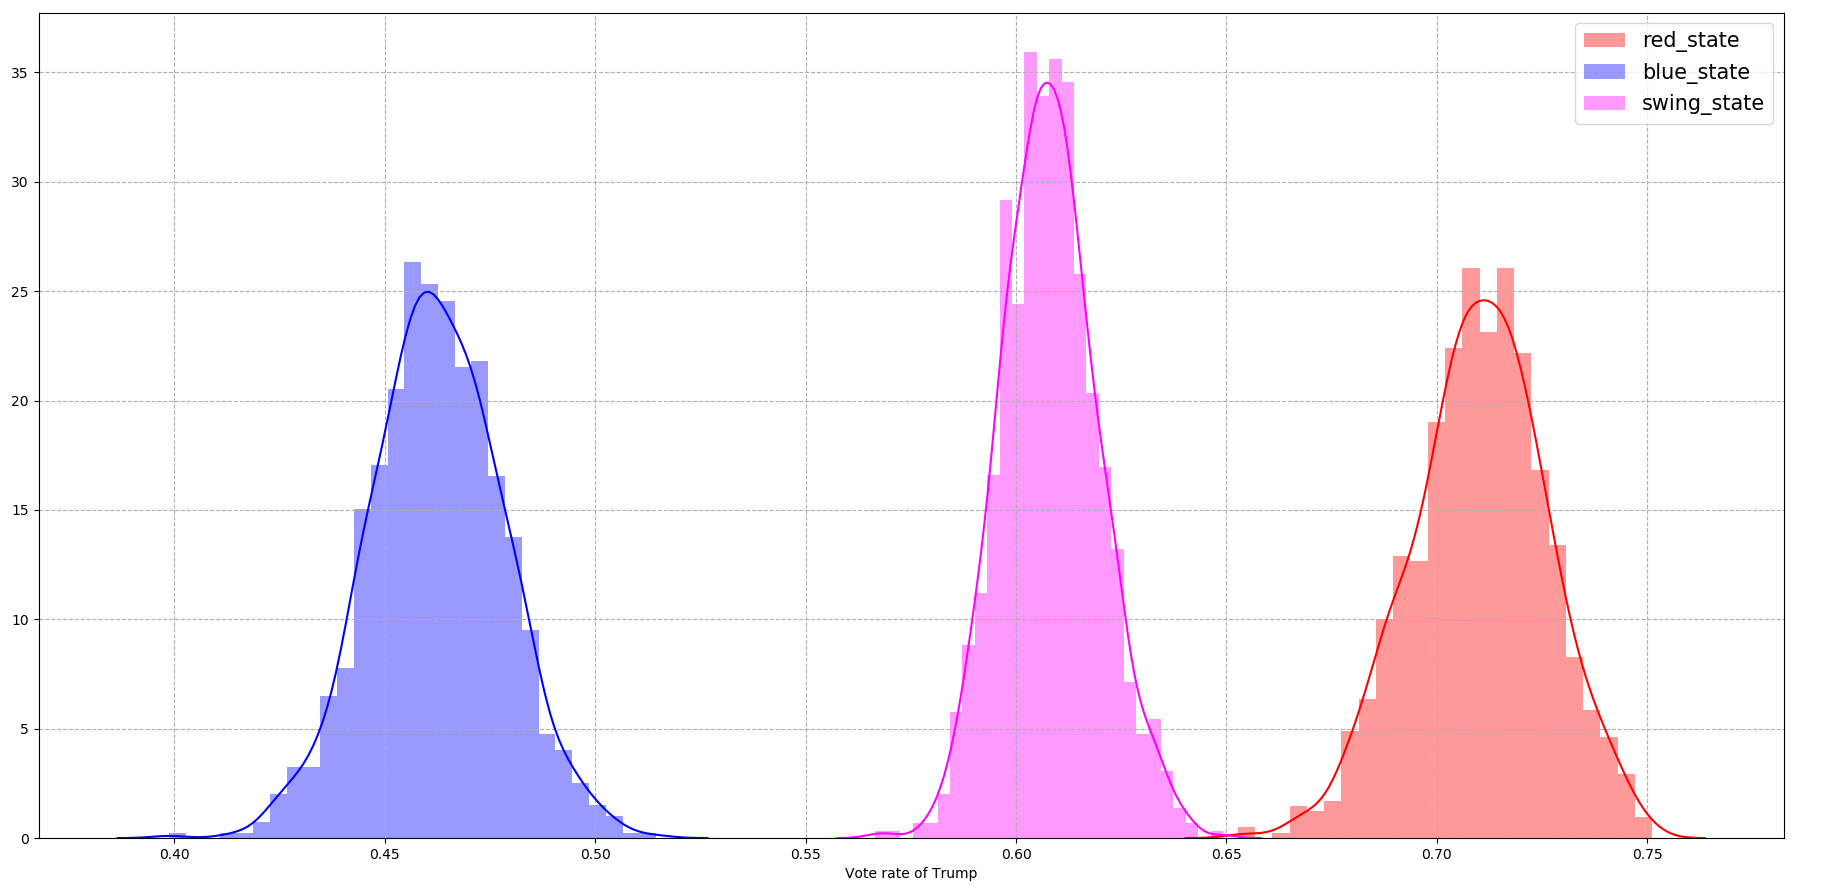
\includegraphics[scale=0.45]{pnt_2.png}
		\caption{样本均值的分布(特朗普)}
		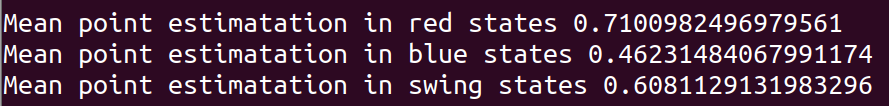
\includegraphics[scale=0.45]{pnt_3.png}
		\caption{点估计结果(特朗普)}
	\end{figure}
	即使在蓝州特朗普也有0.46的得票率均值估计,与希拉里相差不大,而在摇摆州和红州大幅度领先希拉里,看来特朗普真有种众望所归的味道。
		\subsubsection{区间估计}
		获得深红州、深蓝州和摇摆州希拉里得票率均值的置信水平为95\%的置信区间。
		\inputpython{par_estimate.py}{38}{48}
		\begin{figure}[H]
			\centering
			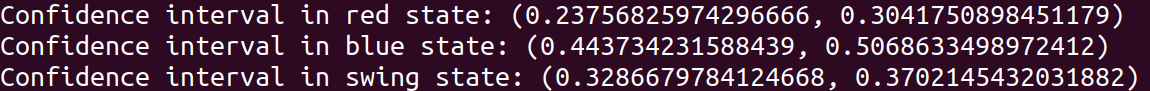
\includegraphics[scale=0.45]{inter.png}
			\caption{区间估计结果}
		\end{figure}
	
	\subsection{假设检验}
	该部分代码位于文件hypo\_test.py中。
		\subsubsection{t检验}
		在EDA中我们发现在深蓝州和深红州希拉里的得票率分布具有较大差异,因此我们有理由判断希拉里在深蓝州得票率的均值$\mu_b$不等于深红州得票率的均值$\mu_r$.现在我们做出假设:
		$$H_0: \mu_b = \mu_r$$
		$$H_1: \mu_b \ne \mu_r$$
		现根据样本进行t检验:
		\inputpython{hypo_test.py}{12}{22}
		\begin{figure}[H]
			\centering
			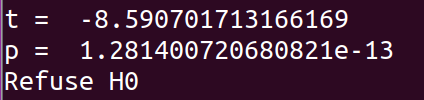
\includegraphics[scale=0.45]{hypo.png}
			\caption{t检验结果}
		\end{figure}
	    根据结果,我们拒绝$H_0$,即我们认为在深蓝州和深红州希拉里得票率不相等。
		\subsubsection{F检验}
		在EDA中可以看出希拉里在深红州和摇摆州得票率曲线比较相似,现通过F检验判断两者方差是否相等。
		$$H_0: \sigma_{swing} = \sigma_{red}$$
		$$H_1: \sigma_{swing} \ne \sigma_{red}$$
		\inputpython{hypo_test.py}{24}{32}
		\begin{figure}[H]
			\centering
			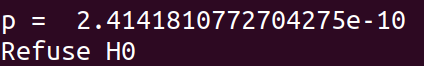
\includegraphics[scale=0.5]{F.png}
			\caption{F检验结果}
		\end{figure}
		由此可见两样本方差并不相等
\section{回归与分类}
	\subsection{线性回归}
	对摇摆州和深蓝州地区的获得学士学位人口比例和希拉里得票率进行线性回归。
	\subsection{朴素贝叶斯分类}
	接下来几节将通过三种机器学习分类方法来对大选结果进行预测,并进行分类性能比较。
		\subsubsection{定义函数classification\_result()}
		该函数参数为训练集和测试集以及分类器,功能是完成模型拟合并输出测试集的分类结果。
	\subsection{决策树分类}
	\subsection{KNN分类}
	\subsection{分类性能比较}
	
\section{总结}


%----------------------------------------------------------------------------------------

\end{document}
